\section{Machine Learning Fundamentals} \label{sec:bt/MLF}

Artificial intelligence is a field of research that has been practiced for a very long time, contrary to popular belief. The first work that is now recognized as AI was written by \textcite{mcculloch1943}. Even still, the concept of artifacts operating under their own control can be traced back to Alexandria ca. 250 BC, where a water regulator was built that could maintain a constant flow rate. Other examples of self-regulating feedback control systems include the steam engine governor and the thermostat, all invented before the 19th-century \cite{russell2009}. This thesis will concentrate on machine learning, a particular form of artificial intelligence that employs prior knowledge of historical data to tackle tasks that are too difficult to solve with fixed programs written and designed by human beings \cite{goodfellow2016}.

% \subsection{Statistical Inference}
\subsection{Learning Algorithms}

A machine learning algorithm is characterized by the fact that it can learn properties from data. \textcite{mitchell1997} famously defines this aspect of learning as "A computer program is said to learn from experience $E$ with respect to some class of tasks $T$ and performance measure $P$, if its performance at tasks in $T$, as measured by $P$, improves with experience $E$." Since machine learning algorithms can be employed in a wide range of problems and trained by an equally wide range of methods, $T$, $P$, and $E$ in this definition can be constructed as just about anything. However, a very common class of tasks $T$ central to this thesis is that of \textit{classification}. The experience $E$ required to train towards this task is usually provided through either \textit{supervised-} or \textit{unsupervised learning}. 

\subsubsection{Classification}

% In the classification task, the computer program is asked to determine which of $k$ discrete categories some input belongs. 
Classification is the task of determining which of $k$ discrete categories some input belongs. Given data (experience $E$) produced by a function $f:\mathbb{R}^{2}\to\{1,\dots,k\}$, a learning algorithm tasked with classification will generate a hypothesis $h:\mathbb{R}^{2}\to\{1,\dots,k\}$ that approximates $f$. Given an input vector $\bm{x}$, $h(\bm{x})$ outputs a probability distribution over possible categories. One popular application is that of object detection, where an image is given as the input $\bm{x}$, and the output is the category to which an object in the image belongs. If $k=2$, the learning problem is called binary classification, and the hypothesis $h$ merely outputs the probability of whether an input represents a single target category or not. Multi-class classification is more common in the general case, however. 

% \subsubsection{The No Free Lunch Theorem}

Since we often cannot assume any prior knowledge of the inherent properties of $f$, choosing a hypothesis $h$ with which to approximate it is no trivial task. We say that $h$ is selected from a \textit{hypothesis space} $\mathcal{H}$, which needs to be defined by the learning algorithm designer. Looking at figure \ref{fig:bt_hypotheses}, one can see the importance of choosing a hypothesis space that is complex enough to approximate $f$ accurately yet simple enough that the function does not overfit. For this example, a 12-degree polynomial is required to produce an approximation that agrees with all the data. However, since we cannot assume that $f$ is not stochastic, this polynomial might generalize poorly to unseen data. In such a case, a simpler hypothesis in a linear or a sinusoidal function might be the optimal choice.

\begin{figure}[h]
    \centering
    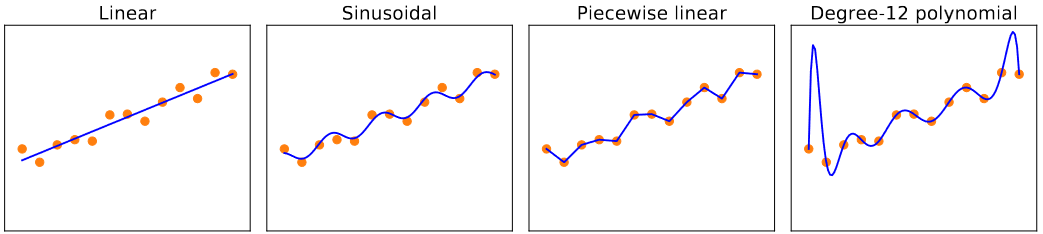
\includegraphics[width=0.8\textwidth]{figures/bt_hypotheses.png}
    \caption{Finding hypotheses to fit data. The four plots each show best-fit functions from four different hypothesis spaces trained on the same dataset.}
    \source{\cite{russell2009}}
    \label{fig:bt_hypotheses}
\end{figure}

\subsubsection{Supervised Learning}

A machine learning algorithm can be called a supervised learning algorithm if it is trained by experiencing a dataset of examples $\bm{x}$, where each example is associated with a target $y$. The training process thus becomes to approximate a function that can reproduce $y$ given $\bm{x}$.

One classic learning algorithm is linear regression, which is supervised learning in its simplest form \cite{goodfellow2016}. The goal of linear regression is to predict a target value $\hat{y}\in\mathbb{R}$ from an $n$-dimensional input vector $\bm{x}\in\mathbb{R}^n$. Since we know then that the output should be a linear function of the input, the problem becomes to approximate the hypothesis given by equation \ref{eq:bt_linReg}. Here $\bm{w}\in\mathbb{R}^n$ is a vector of model parameters, which control the behavior of the system.

\begin{equation}
    \label{eq:bt_linReg}
    h(\bm{x})=\hat{y}=\bm{w}^T\bm{x}
\end{equation}

Now, to determine the optimal value of $\bm{w}$, we need a performance measure $P$. For this particular problem, a typical choice is the \textit{mean squared error} (MSE), given in equation \ref{eq:bt_MSE}. MSE is calculated from a matrix of $m$ input vectors $\bm{X}=\{\bm{x}_1,\dots,\bm{x}_m\}$, their corresponding $m$ target values $\bm{y}=\{y_1,\dots,y_m\}$, and model parameters $\bm{w}$.

\begin{equation}
    \label{eq:bt_MSE}
    MSE=\frac{1}{m}\sum_{i}(\hat{\bm{y}}-\bm{y})^2
    =\frac{1}{m}||\hat{\bm{y}}-\bm{y}||^2_2
\end{equation}

By setting $\hat{\bm{y}}=\bm{y}$, one can see that $MSE=0$, and furthermore that it increases linearly with the euclidean distance between $\hat{\bm{y}}$ and $\bm{y}$. As such, the optimal model parameters can be obtained by minimizing $MSE$ with respect to $\bm{w}$. This can be done by solving for where its gradient is $\bm{0}$, as is in equations \ref{eq:bt_MSE_gradientB} to \ref{eq:bt_MSE_gradientE}.

\begin{equation}
    \label{eq:bt_MSE_gradientB}
    \nabla_{\bm{w}}MSE=\bm{0}
\end{equation}
\begin{equation}
    \Rightarrow \nabla_{\bm{w}}\frac{1}{m}||\hat{\bm{y}}-\bm{y}||^2_2=\bm{0}
\end{equation}
\begin{equation}
    \Rightarrow \nabla_{\bm{w}}\frac{1}{m}||\bm{X}\bm{w}-\bm{y}||^2_2=\bm{0}
\end{equation}
\begin{equation*}
    \vdots
\end{equation*}
\begin{equation}
    \label{eq:bt_MSE_gradientE}
    \Rightarrow \bm{w}=(\bm{X}^T\bm{X})^{-1}\bm{X}^T\bm{y}
\end{equation}

Evaluation of equation \ref{eq:bt_MSE_gradientE} results in a value of $\bm{w}$ which optimally fits the training dataset. As such, it constitutes a simple learning algorithm \cite{goodfellow2016}.

% For object detection, each image in the dataset is accompanied by a value representing the object it displays. 

% \subsection{Decision Tree Classifier}

% Decision tree induction is one of the simplest and yet most successful forms of machine learning (\cite{russell2009}). It is also a supervised learning algorithm, as it requires a dataset of labeled examples to be trained. The Decision Tree Classifier takes a vector of attribute values as input and returns a "decision." It reaches this decision by performing a sequence of tests on one or more attributes. An example is presented in figure \ref{fig:bt_decision_tree}. Here, one can imagine that the species of an animal is to be determined based upon a set of attributes \{"Has feathers?", "Can fly?", "Has finns?"\}. The likely animal species can be determined by following a path from the root node to a leaf node. Although this example is simple, the general principle holds for more complex classification problems as well.

% \begin{figure}[h]
%     \centering
%     \includegraphics[width=0.5\textwidth]{Images/bt_decision_tree.png}
%     \caption{Decision Tree Example. Each internal node represents a test on one attribute, and its branches are labeled with possible attribute values. Leaf nodes represent a decision.}
%     \label{fig:bt_decision_tree}
% \end{figure}

% The training process of decision trees is done with specialized algorithms, the specific details of which are outside the scope of this thesis. However, they are usually based on a greedy divide-and-conquer strategy, where the training dataset is split on whatever attribute is most important. Which attribute this is, and at what attribute value the split is done, is determined by a notion of \textit{information gain}. 

% \subsection{Ensemble Learning}

% Ensemble learning is a relatively straightforward method that has a remarkable effect of reducing generalization error (\cite{goodfellow2016}). When a machine learning model has been trained, one is left with a single hypothesis $h$ that, to a certain degree, is able to approximate some function $f$. However, if the model is trained once more, the resulting approximation would likely produce slightly differing predictions. The notion of ensemble learning is to train multiple independent models and combine their predictions. Specifically, by determining the output by majority voting or an average, the method is termed \textit{model averaging}. 
% Some ensemble methods construct their ensemble of models by random, others by some rationale. \textit{Bootstrap aggregating} (bagging), for example, trains each model on a subset of the original training dataset by sampling at random with replacement. This strategy ensures an inherent distinction between models, which offers a broader hypothesis space and reduced generalization error.